\documentclass[conference]{IEEEtran}
\IEEEoverridecommandlockouts

\usepackage{iftex}
\ifPDFTeX
  \usepackage[utf8]{inputenc}
  \usepackage[T1]{fontenc}
\else
  \usepackage{fontspec}
  \setmainfont{texgyretermes-regular.otf}[BoldFont=texgyretermes-bold.otf, ItalicFont=texgyretermes-italic.otf, BoldItalicFont=texgyretermes-bolditalic.otf]
  \setsansfont{texgyreheros-regular.otf}[BoldFont=texgyreheros-bold.otf, ItalicFont=texgyreheros-italic.otf]
  \setmonofont{texgyrecursor-regular.otf}[BoldFont=texgyrecursor-bold.otf]
\fi
\usepackage[spanish,es-noquoting,es-nodecimaldot,es-tabla]{babel}
\usepackage{amsmath,amssymb}
\usepackage{graphicx}
\usepackage{booktabs}
\usepackage{array}
\usepackage{multirow}
\usepackage{url}
\usepackage[hidelinks]{hyperref}
\usepackage{balance}

\graphicspath{{figures/}{../../reports/figures/}}
\urlstyle{same}

\renewcommand{\IEEEkeywordsname}{Palabras clave}
\newcommand{\gaitndd}{\texttt{gaitndd}}
\newcommand{\gaitpdb}{\texttt{gaitpdb}}

\begin{document}

\title{Dinámica de la marcha para la clasificación de enfermedades neurodegenerativas:\\modelado, evaluación agrupada por sujeto y validación externa}

\author{
\IEEEauthorblockN{Luis Renato Alvarez Ccopa, Andersson Chiroque Silva, David Teofilo Orihuela Serafin,\\
Jeraldine Dione Rojas Vargas, Dayanna Gisell Quispe Gallardo}
\IEEEauthorblockA{\textit{Universidad de Ingeniería y Tecnología (UTEC)}\\
Lima, Perú}
}

\maketitle

\begin{abstract}
Se estudia si la dinámica de la marcha permite clasificar a sujetos sanos y a pacientes con enfermedad de Parkinson (EP), enfermedad de Huntington (EH) y esclerosis lateral amiotrófica (ELA), con el sujeto como unidad de análisis. Se usaron 63 sujetos de la base \textit{Gait in Neurodegenerative Disease} de PhysioNet, de cuyas series de zancada filtradas se calcularon 12 descriptores de ritmo, variabilidad, simetría y estructura temporal. Se compararon dos referencias y cuatro modelos (regresión logística, SVM, bosque aleatorio y gradient boosting), además de un enfoque que entrena con ventanas y decide por sujeto, mediante validación cruzada anidada y agrupada por sujeto, de 5 particiones repetida 10 veces. El bosque obtuvo una exactitud balanceada de $0.605 \pm 0.016$ y el bosque entrenado con ventanas, $0.647 \pm 0.028$ (azar: 0.25; permutación, $p=0.001$), sin diferencias significativas entre modelos. Separar sanos de enfermos es mucho más fácil (0.87) que distinguir entre las tres enfermedades (0.56--0.62); la confusión principal es EP--EH. Edad y sexo solos clasifican con 0.46, lo que confirma el confusor señalado en la primera etapa. Para aislarlo, el clasificador EP--control se transportó sin reentrenar a una segunda cohorte de 165 sujetos con edades comparables (\textit{Gait in Parkinson's Disease}), cuyas zancadas se extrajeron de la fuerza plantar: el modelo de marcha conservó un AUC de 0.71 [0.63, 0.79], mientras que el de edad cayó a 0.52. Se muestra además que variables que dependen de la duración del registro mejoran la validación interna y hacen fallar la externa.
\end{abstract}

\begin{IEEEkeywords}
análisis de marcha, enfermedades neurodegenerativas, clasificación multiclase, validación cruzada anidada, fuga de información, validación externa
\end{IEEEkeywords}

\section{Introducción}

La enfermedad de Parkinson (EP), la enfermedad de Huntington (EH) y la esclerosis lateral amiotrófica (ELA) alteran el control motor por vías distintas: la EP compromete los ganglios basales y produce una marcha lenta y de pasos cortos; la EH genera movimientos coreicos involuntarios; la ELA causa debilidad progresiva por pérdida de motoneuronas. Las tres modifican el ritmo de la marcha, y los trabajos de Hausdorff y colaboradores mostraron que la variabilidad del intervalo de zancada y sus correlaciones de largo alcance cambian en cada una de ellas \cite{hausdorff1997,hausdorff2000,hausdorff2005}. Con sensores de fuerza en el calzado, cinco minutos de marcha bastan para obtener esas series, lo que ha motivado muchos trabajos de clasificación automática sobre estos datos \cite{gaitsurvey2024}.

En la primera entrega (P1) se analizó la cohorte \textit{Gait in Neurodegenerative Disease Database} (\gaitndd) antes de entrenar modelos. Ese análisis dejó tres condiciones para esta etapa. Primero, la unidad de evaluación debe ser el sujeto: particionar al azar ventanas de un mismo individuo inflaba la exactitud balanceada de 0.62 a 0.81. Segundo, el filtrado de artefactos cambia las conclusiones y debe tratarse como una decisión metodológica. Tercero, el grupo control es 27 años más joven que el de EP, de modo que cualquier resultado puede contener un efecto de la edad que \gaitndd{} no permite separar.

Esta segunda entrega (P2) completa el estudio. Se plantea una clasificación supervisada en cuatro clases (control, EP, EH, ELA) con el sujeto como unidad, y se comparan dos referencias y cuatro modelos bajo validación cruzada anidada y agrupada. Las preguntas de investigación son las de P1:

\textbf{PI1.} ¿Los descriptores de marcha permiten distinguir entre las tres enfermedades, o solo separan sanos de enfermos?

\textbf{PI2.} ¿Cuánto optimismo introduce evaluar unidades dependientes (ventanas) en lugar de sujetos, y puede aprovecharse la representación por ventanas sin ese sesgo?

\textbf{PI3.} ¿Qué parte del desempeño se explica por edad, sexo o velocidad de marcha y no por la patología?

Para la PI3 se usa una segunda cohorte, \textit{Gait in Parkinson's Disease Database} (\gaitpdb), en la que la edad casi no difiere entre pacientes y controles. Un modelo entrenado en \gaitndd{} se evalúa en ella sin reentrenar.

\section{Datos y análisis exploratorio}

\subsection{Cohortes}
\gaitndd{} contiene 64 participantes (16 controles, 15 EP, 20 EH y 13 ELA) que caminaron cinco minutos a paso cómodo por un pasillo de 77~m con un sensor de fuerza bajo cada pie, muestreado a 300~Hz \cite{hausdorff2000,goldberger2000}. Además de la señal cruda, la base entrega una serie con 13 medidas por zancada: duración, balanceo, apoyo y apoyo doble, en segundos y como porcentaje del ciclo. En total hay 15\,160 zancadas. La Tabla~\ref{tab:cohorte} resume su composición.

\gaitpdb{} reúne tres estudios con 93 pacientes con EP y 73 controles: Ga, sobre doble tarea \cite{yogev2005}; Ju, sobre estimulación auditiva rítmica \cite{hausdorff2007}; y Si, sobre marcha en caminadora \cite{frenkel2005}. Cada sujeto tiene ocho sensores de fuerza por pie a 100~Hz y caminatas de unos dos minutos. Un control (\texttt{Juc010}) no tiene registros, por lo que se usan 165 sujetos. La base no incluye series de zancada derivadas; la Sección~\ref{sec:prepro} describe cómo se extrajeron.

\begin{table}[t]
\caption{Composición de las cohortes}
\label{tab:cohorte}
\centering
\footnotesize
\begin{tabular}{@{}llrrrr@{}}
\toprule
Cohorte & Grupo & $n$ & Edad & Hombres & Velocidad \\
 & & & (años) & (\%) & (m/s) \\
\midrule
\multirow{4}{*}{\gaitndd} & Control & 16 & 39.3 & 12.5 & 1.35 \\
 & EP & 15 & 66.8 & 66.7 & 1.00 \\
 & EH & 20 & 46.7 & 30.0 & 1.15 \\
 & ELA & 13 & 55.6 & 76.9 & 1.05 \\
\midrule
\multirow{2}{*}{\gaitpdb} & Control & 72 & 63.7 & 55.6 & -- \\
 & EP & 93 & 66.3 & 62.4 & -- \\
\bottomrule
\end{tabular}
\end{table}

\subsection{Calidad de los datos}
La metadata de \gaitndd{} no puede leerse directamente: un salto de línea parte el registro de \texttt{hunt20}, los faltantes están codificados como el texto \texttt{MISSING}, la columna de grupo etiqueta a los 13 sujetos con ELA como \texttt{subjects} y la columna de severidad mezcla cuatro escalas (Hoehn y Yahr en EP \cite{hoehn1967}, capacidad funcional total en EH \cite{shoulson1979}, meses desde el diagnóstico en ELA y cero en controles). Esta última columna identifica la clase y se excluye de los predictores \cite{kaufman2012}. Las tallas y pesos usan convenciones distintas en cada subcohorte y tampoco se usan. La Tabla~\ref{tab:metadata} resume los problemas y su tratamiento.

\begin{table}[t]
\caption{Problemas de la metadata de \gaitndd{} y tratamiento}
\label{tab:metadata}
\centering
\footnotesize
\begin{tabular}{@{}p{0.36\columnwidth}p{0.22\columnwidth}p{0.32\columnwidth}@{}}
\toprule
Problema & Alcance & Tratamiento \\
\midrule
Registro \texttt{hunt20} partido & 65 filas para 64 sujetos & lector propio \\
Texto \texttt{MISSING} & 4 campos & conversión a faltante \\
ELA etiquetada \texttt{subjects} & 13 sujetos & clase desde el identificador \\
Severidad con 4 escalas & todos & excluida (fuga) \\
Talla y peso con unidades mixtas & 3 subcohortes & excluidos \\
Canal derecho de \texttt{hunt20} & 1 sujeto & sujeto excluido \\
\bottomrule
\end{tabular}
\end{table}

Las series de zancada se distribuyen sin filtrar e incluyen intervalos de hasta 55~s (pausas o pisadas no detectadas). Se aplicaron tres reglas fisiológicas: duración entre 0.5 y 2.5~s, apoyo doble no negativo y porcentajes de fase en $[0, 100]$. El sujeto \texttt{hunt20} se excluyó porque su canal derecho no registra despegues (el 100\,\% de sus zancadas viola alguna regla). Quedan 63 sujetos y 14\,732 zancadas. El descarte es desigual: 5.9\,\% de las zancadas en ELA frente a 0.02\,\% en controles.

\subsection{Hallazgos exploratorios}
La Fig.~\ref{fig:eda} resume los hallazgos de P1 que condicionan el modelado. Los grupos difieren en edad y velocidad (paneles a y b), de modo que ambas son confusores potenciales. El filtrado cambia el orden de los grupos (panel c): sin filtrar, el CV medio de ELA es 0.43, diez veces el de los controles; filtrado baja a 0.063 y el grupo más variable pasa a ser EH (0.105). EH tiene además el menor exponente de DFA (panel d), es decir, una serie con menos memoria, como se describe en la literatura \cite{hausdorff1997}. Ningún descriptor aislado separa los cuatro grupos.

\begin{figure*}[t]
\centering
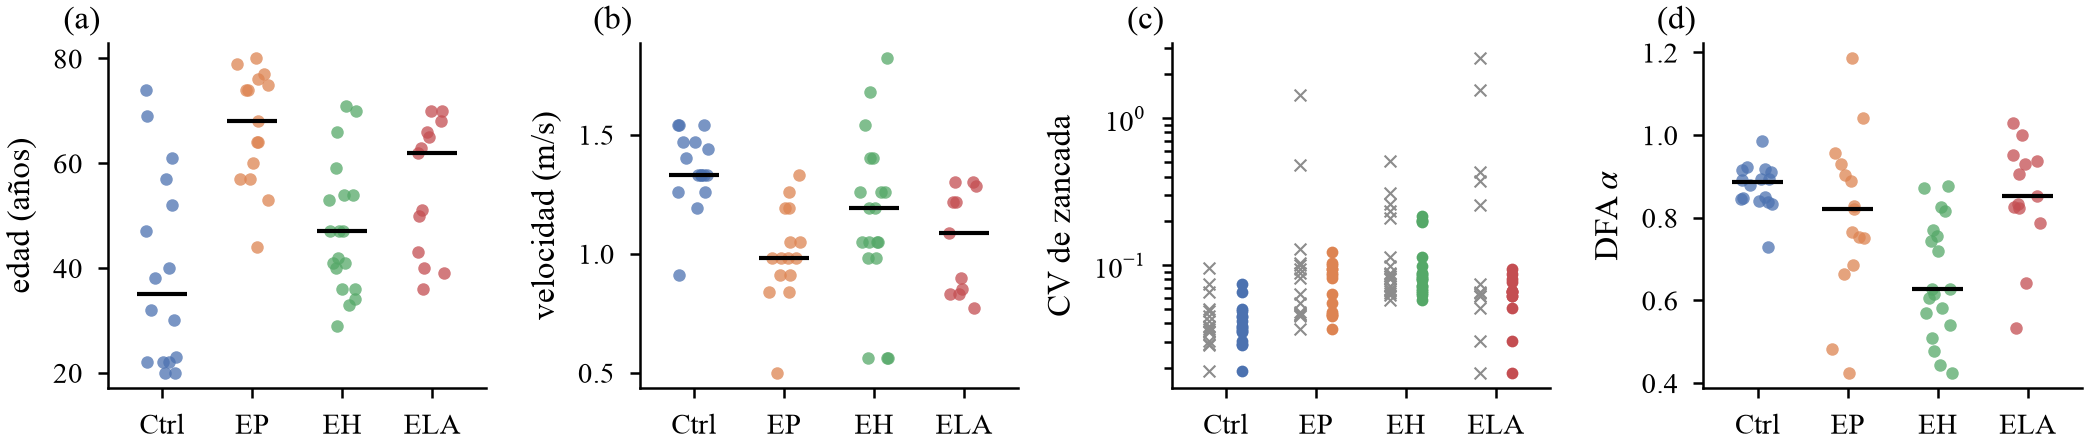
\includegraphics[width=\textwidth]{eda_resumen.png}
\caption{Hallazgos exploratorios en \gaitndd{} (63 sujetos). (a) Edad y (b) velocidad de marcha por grupo. (c) Coeficiente de variación del intervalo de zancada antes (cruces grises) y después (círculos) del filtrado fisiológico, en escala logarítmica. (d) Exponente $\alpha$ de DFA tras el filtrado. Cada punto es un sujeto; la línea horizontal marca la mediana. Ctrl: control; EP: Parkinson; EH: Huntington.}
\label{fig:eda}
\end{figure*}

En P1 también se cuantificó la fuga por sujeto con un bosque aleatorio fijo sobre ventanas de 30 zancadas (Tabla~\ref{tab:fuga}). La partición aleatoria de ventanas dio una exactitud balanceada 19 puntos mayor que la agrupada por sujeto, con los mismos datos y el mismo modelo; la evaluación directa por sujeto coincidió con la agrupada. La diferencia viene de dejar ventanas del mismo individuo a ambos lados de la partición: el modelo reconoce a la persona, no la enfermedad \cite{saeb2017}. Toda la evaluación de este trabajo agrupa por sujeto.

\begin{table}[t]
\caption{Experimento de fuga de P1 (bosque aleatorio fijo)}
\label{tab:fuga}
\centering
\footnotesize
\begin{tabular}{@{}llc@{}}
\toprule
Unidad & Partición & Exactitud bal. \\
\midrule
Ventana de 30 zancadas & aleatoria & $0.812 \pm 0.049$ \\
Ventana de 30 zancadas & agrupada por sujeto & $0.622 \pm 0.086$ \\
Sujeto & estratificada & $0.642 \pm 0.048$ \\
\bottomrule
\end{tabular}
\end{table}

\section{Preprocesamiento e ingeniería de características}
\label{sec:prepro}

\subsection{Descriptores por sujeto}
De cada serie filtrada se calcularon 12 descriptores (Tabla~\ref{tab:descriptores}). Diez provienen de P1. Se agregaron dos. La \textit{variabilidad sucesiva} es la raíz del cuadrado medio de las diferencias entre zancadas consecutivas, dividida por la media; a diferencia del CV, no se ve afectada por cambios lentos de velocidad a lo largo de la caminata. La \textit{entropía muestral} (SampEn, $m=2$, $r=0.2\,\sigma$) mide la regularidad de la serie a escala corta \cite{richman2000} y complementa a DFA, que describe correlaciones a escalas largas \cite{peng1995}. Ambas implementaciones se verificaron con señales de comportamiento conocido (pruebas unitarias del repositorio).

\begin{table}[t]
\caption{Descriptores de marcha usados por los modelos}
\label{tab:descriptores}
\centering
\footnotesize
\begin{tabular}{@{}p{0.2\columnwidth}p{0.71\columnwidth}@{}}
\toprule
Familia & Descriptores \\
\midrule
Ritmo & duración media de zancada \\
Variabilidad & CV, rango intercuartílico, variabilidad sucesiva$^{*}$ \\
Simetría & asimetría izquierda--derecha de duración y de balanceo \\
Estructura temporal & autocorrelación de retardo 1, $\alpha$ de DFA, entropía muestral$^{*}$ \\
Fases del ciclo & CV del balanceo, media y CV del apoyo doble \\
\bottomrule
\multicolumn{2}{@{}l}{\scriptsize $^{*}$ Nuevos en P2.}
\end{tabular}
\end{table}

Se descartaron variables por tres motivos. Por redundancia exacta: la desviación estándar de la zancada es el producto de CV y media, y el balanceo medio tiene $r=-1.00$ con el apoyo doble medio, porque en cada zancada el apoyo doble es lo que resta del ciclo tras ambos balanceos. Por depender del filtrado: el número de zancadas válidas y la cadencia derivada de él disminuyen cuando el filtro descarta más zancadas, lo que ocurre sobre todo en ELA, por lo que codifican en parte la calidad de la detección. Por fuga o falta de comparabilidad: severidad, talla y peso. Edad, sexo y velocidad no entran al modelo principal y se usan para estudiar los confusores.

Persisten correlaciones altas entre descriptores retenidos (CV y variabilidad sucesiva, $r=0.96$; autocorrelación y DFA, $r=0.86$). No se eliminaron a mano, porque esa selección se haría con todos los sujetos, incluidos los de prueba; la redundancia se deja a la regularización de cada modelo.

Las transformaciones que aprenden de los datos se ajustan dentro del pipeline de cada modelo y, por lo tanto, solo con los sujetos de entrenamiento de cada partición: imputación por mediana (solo afecta a la velocidad, que falta en dos sujetos con ELA) y estandarización (solo en los modelos lineales y el SVM).

\subsection{Representación por ventanas}
Para el segundo enfoque de modelado se dividió cada serie en ventanas de 30 zancadas consecutivas, lo que produce 480 ventanas. La entropía muestral no está definida en el 41\,\% de ellas (con 30 puntos a veces no hay plantillas coincidentes), por lo que este enfoque usa los otros 11 descriptores.

\subsection{Extracción de zancadas en \gaitpdb}
A partir de la fuerza total bajo cada pie se marcó contacto cuando la fuerza supera el 5\,\% de su percentil 99 en ese registro; se rellenaron huecos y se eliminaron contactos menores a 0.1~s. Los inicios de contacto son apoyos de talón y los finales, despegues (Fig.~\ref{fig:eventos}). Con estos eventos se construyó una tabla con las mismas columnas que \gaitndd{} y se aplicaron las mismas reglas de calidad, que descartaron menos del 1\,\% de las zancadas. Se usó solo la primera caminata de cada sujeto (sufijo \texttt{\_01}), la de referencia; varias de las siguientes corresponden a condiciones experimentales, como la doble tarea, diseñadas justamente para alterar el ritmo de la marcha \cite{yogev2005,hausdorff2007}, y promediarlas mezclaría condiciones. La mediana resultante es de 103 zancadas por sujeto. Para que entrenamiento y prueba tengan series de largo comparable, los descriptores de \gaitndd{} usados en la validación externa se calcularon sobre los primeros 110~s de cada registro.

\begin{figure}[t]
\centering
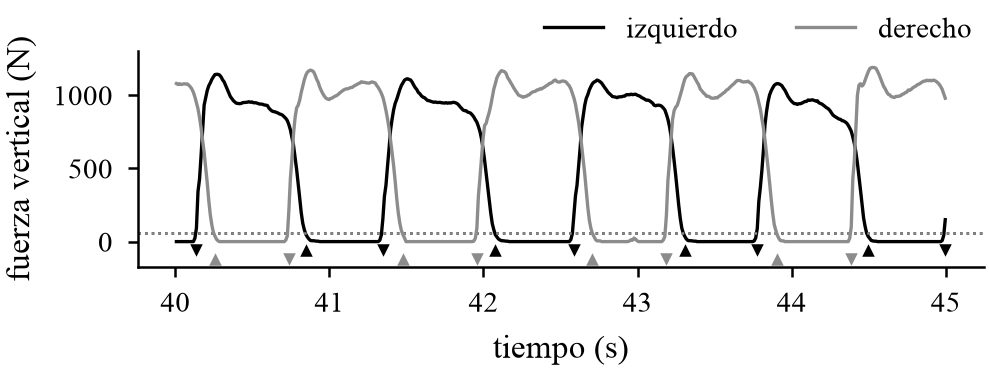
\includegraphics[width=\columnwidth]{deteccion_eventos.png}
\caption{Detección de eventos en el registro \texttt{GaCo01\_01} de \gaitpdb. Líneas: fuerza vertical total bajo cada pie; punteadas: umbral de contacto; triángulos hacia abajo y hacia arriba: apoyos de talón y despegues detectados.}
\label{fig:eventos}
\end{figure}

\section{Metodología y modelos}

\subsection{Modelos de referencia}
Se definieron dos referencias. La \textit{clase mayoritaria} predice siempre EH, el grupo más numeroso, y fija el piso de la exactitud balanceada en 0.25. La segunda es una regresión logística sin ajuste de hiperparámetros que usa solo los dos marcadores clásicos de la literatura, CV y $\alpha$ de DFA \cite{hausdorff1997,hausdorff2000}. Sirve para medir cuánto aportan los otros diez descriptores y los modelos más flexibles.

\subsection{Modelos}
Los cuatro modelos usan los 12 descriptores y pesos de clase inversamente proporcionales a su frecuencia.

\textit{Regresión logística multinomial} con penalización elastic net \cite{zou2005}. Con 63 sujetos es el candidato natural: tiene pocos parámetros, la penalización $L_1$ selecciona variables y la $L_2$ reparte el peso entre descriptores correlacionados, y sus coeficientes se pueden leer.

\textit{Máquina de vectores de soporte} con kernel RBF \cite{cortes1995}, que permite fronteras no lineales controladas por dos hiperparámetros. Sus probabilidades se obtienen con calibración sigmoide \cite{platt1999} en tres particiones internas.

\textit{Bosque aleatorio} de 300 árboles \cite{breiman2001}. Capta interacciones entre descriptores, no requiere escalamiento y el submuestreo de variables reduce el efecto de la redundancia.

\textit{Gradient boosting} \cite{friedman2001} con submuestreo de 0.8, para evaluar si un ensamble secuencial aprovecha estructura que el bosque no ve, a costa de mayor riesgo de sobreajuste con pocos datos.

La Tabla~\ref{tab:grilla} muestra el espacio de búsqueda de cada modelo. Las grillas son pequeñas a propósito: con unos 50 sujetos de entrenamiento por partición, una búsqueda amplia selecciona combinaciones por ruido \cite{cawley2010}.

\begin{table}[t]
\caption{Espacio de búsqueda de hiperparámetros}
\label{tab:grilla}
\centering
\footnotesize
\begin{tabular}{@{}lll@{}}
\toprule
Modelo & Hiperparámetro & Valores \\
\midrule
Logística & $C$ & 0.01, 0.03, 0.1, 0.3, 1, 3, 10 \\
 & proporción $L_1$ & 0, 0.5, 1 \\
SVM & $C$ & 0.3, 1, 3, 10, 30 \\
 & $\gamma$ & \texttt{scale}, 0.01, 0.03, 0.1 \\
Bosque & profundidad máx. & sin límite, 4 \\
 & mín. por hoja & 1, 3, 5 \\
 & variables por división & $\sqrt{p}$, $0.5\,p$ \\
Boosting & árboles & 100, 300 \\
 & tasa de aprendizaje & 0.03, 0.1 \\
 & profundidad & 1, 2, 3 \\
\bottomrule
\end{tabular}
\end{table}

\subsection{Segundo enfoque: entrenamiento por ventanas}
La regresión logística y el bosque se entrenaron también sobre ventanas de 30 zancadas. Las particiones se definen sobre sujetos, la validación interna agrupa las ventanas por sujeto y, para cada sujeto de prueba, se promedian las probabilidades de sus ventanas antes de asignar la clase. El modelo dispone de unas ocho veces más filas de entrenamiento, pero cada sujeto cuenta una sola vez en la evaluación. Este enfoque responde la segunda parte de la PI2.

\section{Diseño experimental y evaluación}

\subsection{Validación cruzada anidada}
La evaluación usa validación cruzada estratificada de cinco particiones sobre los 63 sujetos, repetida diez veces con semillas distintas (50 pares entrenamiento/prueba con 50 o 51 sujetos de entrenamiento y 12 o 13 de prueba). En cada partición de entrenamiento, una búsqueda en grilla con cinco particiones internas, estratificadas y agrupadas por sujeto, elige los hiperparámetros por exactitud balanceada; el modelo se reentrena con todo el entrenamiento y solo entonces predice la partición de prueba \cite{cawley2010,varoquaux2018}. Cada repetición produce una predicción fuera de muestra por sujeto. Las métricas se calculan por repetición sobre los 63 sujetos y se informan como media $\pm$ desviación estándar entre repeticiones. Todos los modelos usan las mismas 50 particiones, de modo que sus diferencias son pareadas. La implementación usa scikit-learn \cite{pedregosa2011}.

\subsection{Métricas}
La métrica principal es la \textit{exactitud balanceada},
\begin{equation}
\mathrm{BA} = \frac{1}{K}\sum_{k=1}^{K}\frac{TP_k}{TP_k+FN_k},
\label{eq:ba}
\end{equation}
con $K=4$ clases. Al promediar la sensibilidad de cada clase no depende de que EH tenga más sujetos, y su valor de azar es $1/K = 0.25$. Se informan también el $F_1$ macro, $F_{1,\mathrm{macro}} = \frac{1}{K}\sum_k F_{1,k}$, que penaliza además las falsas alarmas de cada clase; el AUC macro uno contra el resto, que evalúa el orden de las probabilidades sin fijar umbral; y la sensibilidad por clase. Para analizar qué pares de grupos se distinguen se calculó, para cada par $(a, b)$, el AUC de $p_a/(p_a+p_b)$ entre los sujetos de esos dos grupos \cite{hand2001}.

\subsection{Pruebas estadísticas}
Las diferencias entre modelos se evaluaron con la prueba $t$ corregida para remuestreo de Nadeau y Bengio \cite{nadeau2003}, que corrige la varianza por el solapamiento entre conjuntos de entrenamiento de distintas particiones. Para verificar que el mejor modelo supera el azar se usó una prueba de permutación con 1000 barajados de las etiquetas \cite{ojala2010}; por costo computacional, en ella los hiperparámetros se fijaron en la combinación más elegida por la validación interna.

\subsection{Análisis complementarios}
\textit{Tareas jerárquicas (PI1).} Se repitió la validación anidada para dos tareas: control frente a paciente (63 sujetos) y diagnóstico diferencial entre EP, EH y ELA (47 pacientes, azar 0.33).

\textit{Confusores (PI3).} Con el mismo esquema se entrenaron modelos con edad y sexo, con velocidad, y con la combinación de estas variables con los descriptores de marcha.

\textit{Validación externa (PI3).} Se entrenó un clasificador EP frente a control con los 31 sujetos de esos grupos en \gaitndd{} (hiperparámetros elegidos por validación interna) y se aplicó sin cambios a los 165 sujetos de \gaitpdb. Se usaron dos conjuntos de variables fijados de antemano: los ocho descriptores que dependen solo de los instantes de apoyo de talón, robustos al cambio de sensor (conjunto principal), y los 12 descriptores. Como contraste se entrenaron modelos con solo edad y con edad y sexo. La métrica principal es el AUC con intervalo bootstrap estratificado de 2000 remuestreos, porque un cambio de dominio puede correr el umbral de decisión aunque el orden de los sujetos se conserve \cite{collins2015}.

\textit{Sensibilidad.} Se repitió la evaluación cambiando una decisión a la vez: nivel de filtrado (ninguno, fisiológico, fisiológico más mediana $\pm 4$ MAD), pie usado para los descriptores temporales (izquierdo, derecho, promedio) y largo de ventana (20, 30 y 60 zancadas). En \gaitpdb{} se repitió la extracción con umbrales de contacto de 2, 10 y 20\,\% del percentil 99 y con un umbral fijo de 50~N, aplicando los mismos modelos ya entrenados.

\textit{Versión preliminar con 19 descriptores.} Una primera versión del modelado usó los 19 descriptores de P1, que incluyen número de zancadas, duración observada y cadencia, con una sola validación cruzada de cinco particiones. Ese análisis se repitió con el protocolo anidado de diez repeticiones, dentro de \gaitndd{} y en la validación externa, para medir el efecto de esas tres variables y el de usar una sola partición.

\section{Resultados y análisis}

\subsection{Comparación de modelos}
La Tabla~\ref{tab:resultados} y la Fig.~\ref{fig:comparacion} resumen la validación anidada. Los cuatro modelos superan con claridad a la clase mayoritaria y quedan entre 0.54 y 0.61 de exactitud balanceada. El bosque aleatorio obtuvo la media más alta ($0.605 \pm 0.016$) y la menor variación entre repeticiones; la regresión logística quedó cerca ($0.591 \pm 0.041$). El SVM no superó a la referencia de dos variables, sobre todo porque casi no reconoce la EP (sensibilidad 0.17). En todos los modelos la EP es la clase más difícil y el control la más fácil.

\begin{table*}[t]
\caption{Resultados de la validación cruzada anidada (media $\pm$ DE entre 10 repeticiones; 63 sujetos)}
\label{tab:resultados}
\centering
\footnotesize
\begin{tabular}{@{}lccccccc@{}}
\toprule
 & & & & \multicolumn{4}{c}{Sensibilidad por clase} \\
\cmidrule(l){5-8}
Modelo & Exactitud bal. & $F_1$ macro & AUC & Ctrl & EP & EH & ELA \\
\midrule
Clase mayoritaria & $0.250 \pm 0.000$ & $0.116 \pm 0.000$ & $0.500 \pm 0.000$ & 0.00 & 0.00 & 1.00 & 0.00 \\
LR sobre CV y DFA & $0.538 \pm 0.034$ & $0.519 \pm 0.036$ & $0.735 \pm 0.017$ & 0.88 & 0.25 & 0.67 & 0.35 \\
\midrule
Regresión logística & $0.591 \pm 0.041$ & $0.583 \pm 0.045$ & $0.812 \pm 0.026$ & 0.82 & 0.37 & 0.66 & 0.52 \\
SVM (RBF) & $0.537 \pm 0.026$ & $0.508 \pm 0.025$ & $0.783 \pm 0.022$ & 0.86 & 0.17 & 0.65 & 0.48 \\
Bosque aleatorio & $\mathbf{0.605 \pm 0.016}$ & $\mathbf{0.595 \pm 0.018}$ & $\mathbf{0.829 \pm 0.018}$ & 0.88 & 0.37 & 0.66 & 0.52 \\
Gradient boosting & $0.566 \pm 0.049$ & $0.560 \pm 0.053$ & $0.763 \pm 0.026$ & 0.79 & 0.39 & 0.66 & 0.42 \\
\midrule
Logística, por sujeto$^{*}$ & $0.588 \pm 0.052$ & $0.572 \pm 0.056$ & $0.810 \pm 0.036$ & 0.89 & 0.33 & 0.60 & 0.54 \\
Logística, por ventanas$^{*}$ & $0.641 \pm 0.030$ & $0.625 \pm 0.031$ & $0.824 \pm 0.013$ & 0.82 & 0.47 & 0.49 & 0.78 \\
Bosque, por sujeto$^{*}$ & $0.613 \pm 0.029$ & $0.603 \pm 0.029$ & $0.823 \pm 0.020$ & 0.88 & 0.37 & 0.68 & 0.53 \\
Bosque, por ventanas$^{*}$ & $\mathbf{0.647 \pm 0.028}$ & $\mathbf{0.631 \pm 0.029}$ & $\mathbf{0.862 \pm 0.016}$ & 0.92 & 0.43 & 0.57 & 0.67 \\
\bottomrule
\multicolumn{8}{@{}l}{\scriptsize $^{*}$ Con los 11 descriptores definidos en ventanas de 30 zancadas (sin entropía muestral); la evaluación es siempre por sujeto.}
\end{tabular}
\end{table*}

\begin{figure}[t]
\centering
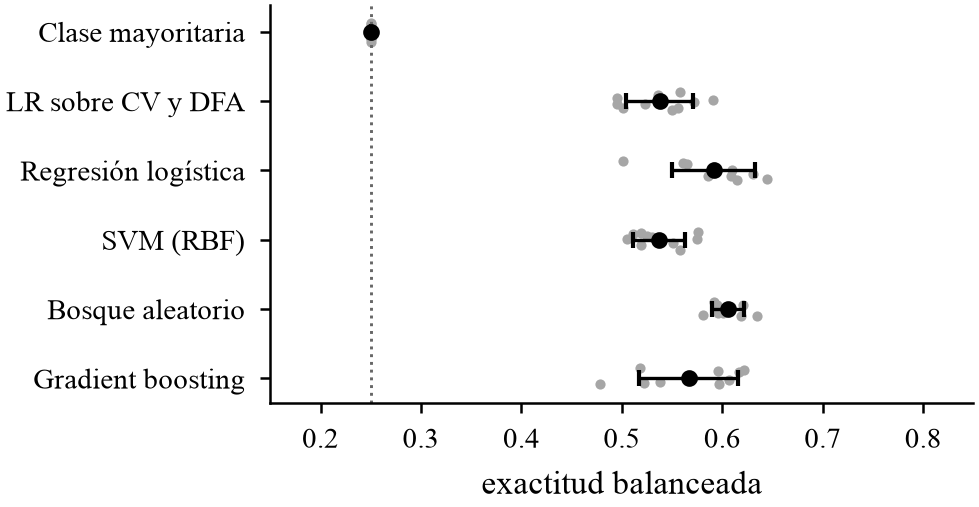
\includegraphics[width=\columnwidth]{comparacion_modelos.png}
\caption{Exactitud balanceada por repetición de la validación anidada (puntos grises, 63 predicciones fuera de muestra cada uno), media y desviación estándar (negro). La línea punteada marca el azar.}
\label{fig:comparacion}
\end{figure}

Ninguna diferencia entre modelos fue significativa con la prueba $t$ corregida, ni siquiera la del bosque frente a la referencia de dos variables ($+0.069$, $p=0.38$). Con 12 o 13 sujetos de prueba, un solo error en una clase de tres sujetos mueve la exactitud balanceada de esa partición en 0.08. Sí es claro que los modelos superan el azar: en la prueba de permutación del bosque ninguna de las 1000 permutaciones alcanzó el valor observado (0.633 frente a un máximo de 0.463; $p=0.001$).

La selección de hiperparámetros fue inestable en los modelos lineales. La logística eligió 14 combinaciones distintas en 50 particiones, la más frecuente solo 5 veces, casi siempre con $C$ entre 0.03 y 3: muchas combinaciones rinden parecido. El bosque fue más estable: la misma combinación (sin límite de profundidad, un sujeto por hoja, $\sqrt{p}$ variables) se eligió 20 veces.

\subsection{Entrenamiento por ventanas (PI2)}
Entrenar con ventanas de 30 zancadas y decidir por sujeto mejoró la media de los dos modelos ($0.588 \rightarrow 0.641$ en la logística y $0.613 \rightarrow 0.647$ en el bosque; Tabla~\ref{tab:resultados}), aunque sin significancia ($p \approx 0.5$). El valor es comparable al 0.62 de la partición agrupada de P1 y muy inferior al 0.81 de la partición aleatoria. La diferencia con P1 es que aquí la mejora no puede venir de fuga, porque ningún sujeto de prueba tiene ventanas en el entrenamiento: el modelo aprovecha la variación de cada sujeto entre ventanas como si fuera un aumento de datos. La respuesta a la PI2 tiene entonces dos partes: evaluar ventanas como observaciones independientes infla la exactitud en 19 puntos, pero entrenar con ventanas y evaluar por sujeto es legítimo y puede ayudar.

\subsection{Qué clases se confunden (PI1)}
La Fig.~\ref{fig:confusion} muestra la matriz de confusión del bosque y la separabilidad por pares. Los controles se distinguen bien de cualquier enfermedad (AUC por pares de 0.89 a 0.98). El par más difícil es EP--EH (0.70): el 39\,\% de las predicciones de los sujetos con EP fueron EH, más que las correctas (37\,\%). ELA se confunde con control en un 25\,\% de los casos.

\begin{figure}[t]
\centering
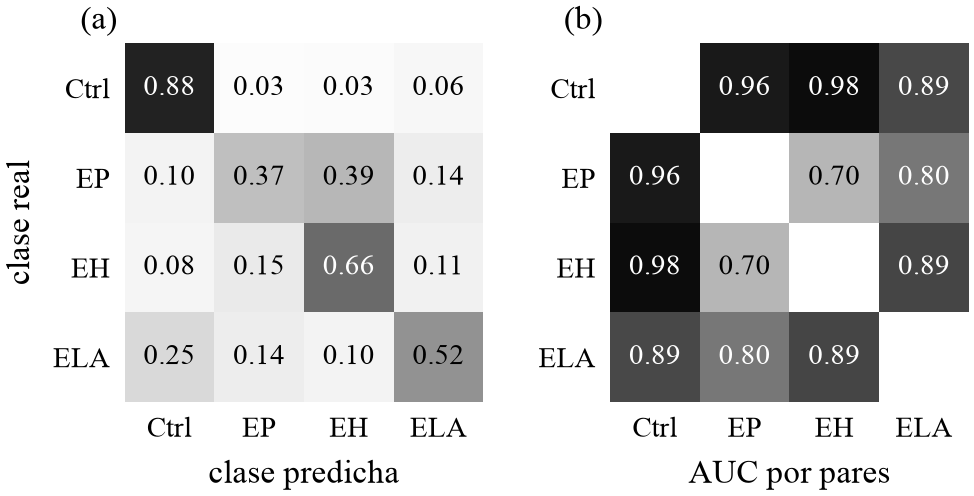
\includegraphics[width=\columnwidth]{confusion_y_pares.png}
\caption{Bosque aleatorio. (a) Matriz de confusión acumulada sobre las 10 repeticiones y normalizada por fila. (b) AUC por pares de clases, calculado con $p_a/(p_a+p_b)$ entre los sujetos de cada par.}
\label{fig:confusion}
\end{figure}

Las tareas jerárquicas (Tabla~\ref{tab:jerarquia}) precisan la respuesta. Separar control de paciente alcanza una exactitud balanceada de 0.86 a 0.87 (AUC 0.92 a 0.94; sensibilidad 0.89, especificidad 0.83). El diagnóstico diferencial entre las tres enfermedades baja a 0.56--0.62, todavía muy por encima del azar de 0.33. La marcha contiene información para distinguir entre patologías, aunque mucho menos que para detectar que existe una.

\begin{table}[t]
\caption{Tareas jerárquicas y conjuntos de variables (validación anidada $5 \times 10$; exactitud balanceada)}
\label{tab:jerarquia}
\centering
\footnotesize
\begin{tabular}{@{}lccc@{}}
\toprule
Tarea o variables & Azar & Logística & Bosque \\
\midrule
Control vs. paciente & 0.50 & $0.866 \pm 0.023$ & $0.860 \pm 0.027$ \\
Diferencial EP/EH/ELA & 0.33 & $0.619 \pm 0.079$ & $0.561 \pm 0.062$ \\
Cuatro clases & 0.25 & $0.591 \pm 0.041$ & $0.605 \pm 0.016$ \\
\midrule
\multicolumn{4}{@{}l}{\textit{Cuatro clases, según variables}} \\
Edad y sexo & 0.25 & $0.462 \pm 0.041$ & $0.439 \pm 0.038$ \\
Velocidad & 0.25 & $0.400 \pm 0.026$ & $0.524 \pm 0.048$ \\
Marcha & 0.25 & $0.591 \pm 0.041$ & $0.605 \pm 0.016$ \\
Marcha, edad y sexo & 0.25 & $0.665 \pm 0.044$ & $0.659 \pm 0.046$ \\
Marcha, edad, sexo y vel. & 0.25 & $0.670 \pm 0.039$ & $0.678 \pm 0.031$ \\
\bottomrule
\end{tabular}
\end{table}

\subsection{Análisis de errores}
De los 63 sujetos, 29 se clasificaron bien en las diez repeticiones y 14 se fallaron en todas. La Fig.~\ref{fig:errores} relaciona la tasa de acierto de cada paciente con su severidad clínica, que no entra al modelo. En EH la relación es fuerte ($\rho=-0.76$): los pacientes con mayor capacidad funcional, es decir, los más leves, se fallan casi siempre. En EP no hay relación con Hoehn y Yahr, porque los errores son de dos tipos. El caso más leve (Hoehn y Yahr 1.5, $\alpha=1.19$) se clasifica como control, mientras que cinco de los otros seis fallos van a EH y tienen un CV de 0.064 a 0.103, muy por encima de la mediana de los controles (0.04). Su variabilidad se parece más a la de la corea que a la del Parkinson típico de la muestra.

\begin{figure*}[t]
\centering
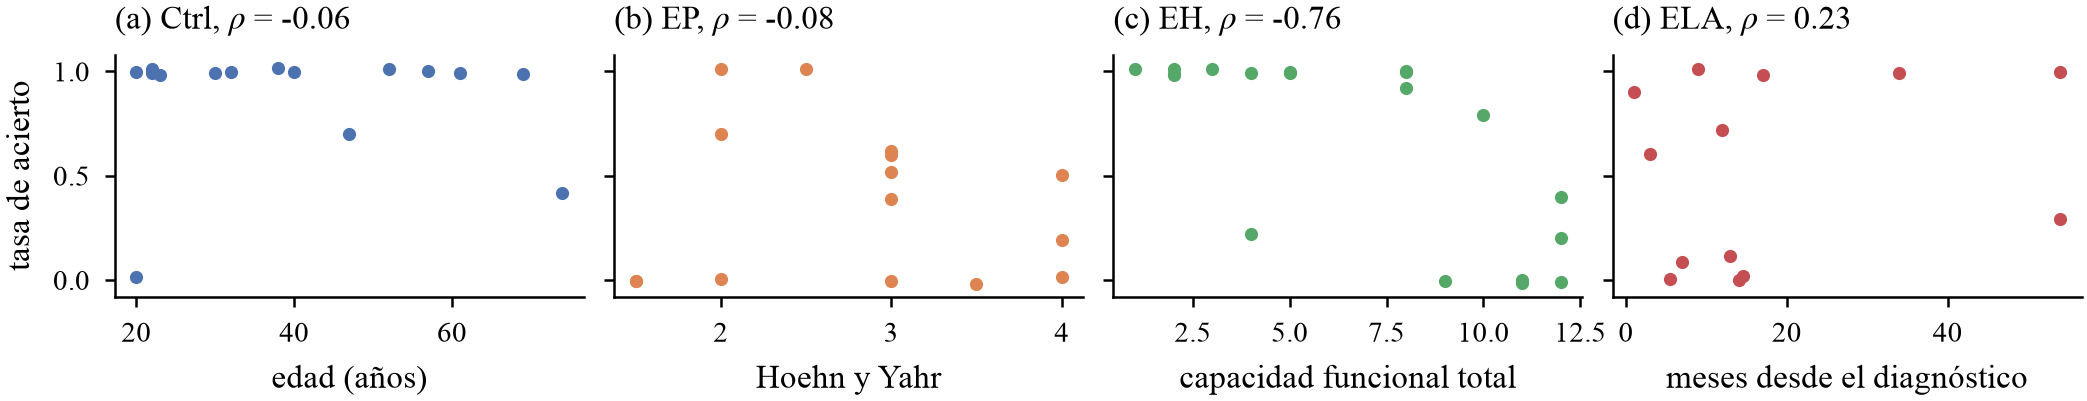
\includegraphics[width=\textwidth]{errores_severidad.png}
\caption{Tasa de acierto por sujeto en las 10 repeticiones (bosque aleatorio) frente a una variable clínica de cada grupo: (a) edad en controles, (b) estadio de Hoehn y Yahr en EP, (c) capacidad funcional total en EH (menor es más grave), (d) meses desde el diagnóstico en ELA. $\rho$: correlación de Spearman.}
\label{fig:errores}
\end{figure*}

\subsection{Importancia de los descriptores}
La Fig.~\ref{fig:importancia} muestra la importancia por permutación calculada sobre los sujetos de prueba de cada partición. Para ambos modelos el descriptor más importante es la duración media de la zancada (0.11 en la logística y 0.07 en el bosque). La logística usa además el apoyo doble medio (0.09) y las medidas de variabilidad; el bosque, el CV del balanceo y el IQR. DFA y la entropía muestral aportan poco por sí solos. Las diferencias entre modelos en las medidas de variabilidad se explican por su correlación: el bosque puede sustituir una por otra y la permutación de cada una por separado no cambia su desempeño \cite{strobl2008}. Los coeficientes de la logística (reentrenada con todos los sujetos) tienen signos coherentes con la clínica: ELA se asocia con zancadas largas y más apoyo doble; EH, con más variabilidad y menor $\alpha$; el control, con menos variabilidad.

\begin{figure}[t]
\centering
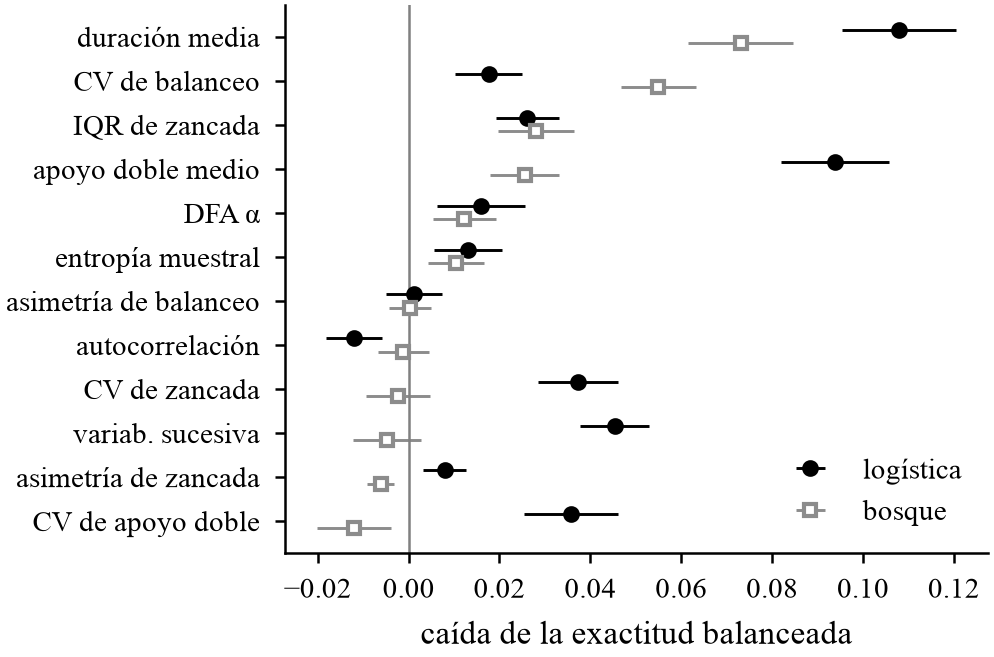
\includegraphics[width=\columnwidth]{importancia_permutacion.png}
\caption{Importancia por permutación (caída de la exactitud balanceada) promediada sobre las 50 particiones externas, con su error estándar.}
\label{fig:importancia}
\end{figure}

\subsection{Confusores dentro de \gaitndd{} (PI3)}
La parte inferior de la Tabla~\ref{tab:jerarquia} muestra que edad y sexo, sin ningún dato de marcha, clasifican con 0.44--0.46, y la velocidad sola con 0.40--0.52. La marcha rinde más (0.59--0.61) y agregarle la demografía sube a 0.66--0.68. Ninguna de estas diferencias es significativa ($p$ entre 0.06 y 0.32). Dentro de \gaitndd{} la demografía ya separa bastante los grupos y no es posible saber cuánto de la señal de marcha es edad.

\subsection{Validación externa en \gaitpdb{} (PI3)}
La Tabla~\ref{tab:externa} y la Fig.~\ref{fig:roc} resumen el transporte del eje EP--control. Los modelos que solo usan la edad separan EP de control dentro de \gaitndd{} con AUC de 0.74 a 0.85, pero en \gaitpdb, donde la edad casi no difiere, caen a 0.52--0.59, con intervalos que tocan o incluyen 0.5. Los modelos con tiempos de zancada también pierden (de 0.81--0.94 a 0.68--0.71), pero sus intervalos quedan por encima de 0.6. Como referencia, entrenar y evaluar dentro de \gaitpdb{} con los mismos ocho descriptores da un AUC de 0.69--0.71: el modelo transportado desde 31 sujetos de otra cohorte y otro sensor ordena a los sujetos casi igual que uno entrenado en la propia cohorte.

\begin{table}[t]
\caption{Transporte del clasificador EP vs. control de \gaitndd{} a \gaitpdb}
\label{tab:externa}
\centering
\footnotesize
\begin{tabular}{@{}llccc@{}}
\toprule
Variables & Modelo & AUC int. & AUC externa [IC 95\,\%] & BA ext. \\
\midrule
Tiempos (8) & Logística & 0.81 & 0.68 [0.60, 0.76] & 0.61 \\
 & Bosque & 0.94 & 0.71 [0.63, 0.79] & 0.66 \\
Todos (12) & Logística & 0.90 & 0.73 [0.65, 0.80] & 0.65 \\
 & Bosque & 0.94 & 0.77 [0.70, 0.84] & 0.66 \\
Edad & Logística & 0.85 & 0.59 [0.51, 0.68] & 0.61 \\
 & Bosque & 0.74 & 0.52 [0.43, 0.61] & 0.50 \\
Edad y sexo & Logística & 0.86 & 0.58 [0.50, 0.67] & 0.54 \\
 & Bosque & 0.82 & 0.57 [0.48, 0.65] & 0.49 \\
\bottomrule
\multicolumn{5}{@{}l}{\scriptsize AUC int.: validación anidada dentro de \gaitndd. BA ext.: exactitud balanceada}\\
\multicolumn{5}{@{}l}{\scriptsize con umbral 0.5 en \gaitpdb.}
\end{tabular}
\end{table}

\begin{figure}[t]
\centering
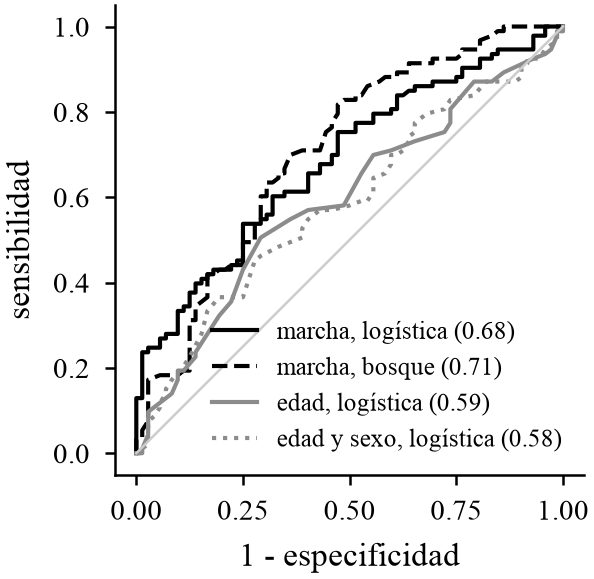
\includegraphics[width=0.62\columnwidth]{roc_externa.png}
\caption{Curvas ROC en \gaitpdb{} (165 sujetos) de modelos entrenados solo con \gaitndd. Entre paréntesis, el AUC.}
\label{fig:roc}
\end{figure}

Con los 12 descriptores el AUC externo es mayor (0.73--0.77), pero el umbral queda desplazado: la sensibilidad sube a 0.83--0.85 y la especificidad baja a 0.44--0.50, lo esperable si el apoyo doble se mide de forma distinta en los dos sistemas. Por estudio de origen, el transporte fue mejor en Si (AUC 0.75--0.87) que en Ga y Ju (0.60--0.76). Cambiar el umbral de contacto entre el 2 y el 20\,\% del percentil 99, o usar 50~N fijos, movió el AUC de los modelos de tiempos de zancada entre 0.64 y 0.73. En cambio, el apoyo doble mediano pasó de 30 a 17\,\%, y el AUC del modelo con todos los descriptores bajó de 0.78 a 0.72. Este resultado justifica haber elegido de antemano los tiempos de zancada como conjunto principal.

\subsection{Versión preliminar con 19 descriptores}
La Tabla~\ref{tab:p1} compara la versión preliminar, que usaba los 19 descriptores de P1, con el conjunto final. La desviación de la exactitud entre las cinco particiones de una misma validación cruzada fue de 0.12 a 0.15, con particiones de hasta 0.94. Por eso un valor de 0.725 obtenido con una sola validación cruzada es posible, aunque el mismo bosque promedia 0.628 en diez repeticiones. Las tres variables de duración aportan dentro de \gaitndd{}: quitarlas baja la logística de 0.668 a 0.618, y el número de zancadas es el tercer descriptor más importante del bosque. Los 12 descriptores finales no mejoran a los 16 de P1 sin duración.

En la validación externa esas variables tienen el efecto contrario. El número de zancadas vale 250 en \gaitndd{} y 103 en \gaitpdb{} solo porque los registros duran cinco y dos minutos. Con los 19 descriptores, la logística predice EP en el 1.8\,\% de los sujetos de \gaitpdb{} y el SVM en el 100\,\%, ambos con exactitud balanceada de 0.50, aunque el AUC de la logística es 0.76: el orden se conserva y lo que falla es el umbral. Recortar \gaitndd{} a 110~s o quitar las tres variables lleva la exactitud balanceada a 0.63--0.70.

\begin{table}[t]
\caption{Efecto de las variables de duración (19 descriptores de P1)}
\label{tab:p1}
\centering
\footnotesize
\begin{tabular}{@{}lcccc@{}}
\toprule
 & \multicolumn{2}{c}{Interna (BA)} & \multicolumn{2}{c}{Externa, logística} \\
\cmidrule(lr){2-3}\cmidrule(l){4-5}
Variables & Logíst. & Bosque & BA & \% pred. EP \\
\midrule
19 de P1 & 0.668 & 0.628 & 0.52 & 1.8 \\
19 de P1, 110~s & -- & -- & 0.63 & 52.1 \\
16 sin duración & 0.618 & 0.603 & 0.70 & 47.9 \\
12 finales & 0.591 & 0.605 & -- & -- \\
8 tiempos, 110~s & -- & -- & 0.61 & 51.5 \\
\bottomrule
\end{tabular}
\end{table}

\subsection{Sensibilidad al preprocesamiento}
La Tabla~\ref{tab:sensibilidad} muestra el efecto de cambiar una decisión a la vez en el bosque. Ninguna variante se aleja más de 0.04 del valor principal, el mismo orden que la desviación entre repeticiones. Llama la atención que sin filtro el desempeño no cambie (0.611). Eso no significa que el filtrado sobre: sin él, los descriptores de ELA y EP incluyen pausas y fallos del sensor, que son más frecuentes en pacientes y por eso también discriminan. El modelo estaría usando errores de detección como síntoma.

\begin{table}[t]
\caption{Sensibilidad del bosque aleatorio a decisiones de preprocesamiento}
\label{tab:sensibilidad}
\centering
\footnotesize
\begin{tabular}{@{}llcc@{}}
\toprule
Decisión & Opción & Exactitud bal. & AUC \\
\midrule
Filtrado & ninguno & $0.611 \pm 0.048$ & 0.833 \\
 & fisiológico (usado) & $0.605 \pm 0.016$ & 0.829 \\
 & fisiológico + MAD & $0.638 \pm 0.025$ & 0.835 \\
Pie & izquierdo (usado) & $0.605 \pm 0.016$ & 0.829 \\
 & derecho & $0.598 \pm 0.026$ & 0.828 \\
 & promedio & $0.623 \pm 0.022$ & 0.839 \\
Ventana$^{*}$ & 20 zancadas & $0.645 \pm 0.033$ & 0.848 \\
 & 30 zancadas & $0.647 \pm 0.018$ & 0.853 \\
 & 60 zancadas & $0.603 \pm 0.023$ & 0.818 \\
\bottomrule
\multicolumn{4}{@{}l}{\scriptsize $^{*}$ Enfoque por ventanas, primeras 5 repeticiones.}
\end{tabular}
\end{table}

\section{Discusión y limitaciones}

\subsection{Interpretación de los resultados}
Con 63 sujetos, la diferencia entre modelos razonables es menor que la incertidumbre de la propia evaluación. El bosque y la logística rinden casi igual y ninguno se separa estadísticamente de una logística con dos variables. El bosque tuvo la menor variación entre repeticiones, probablemente porque el promedio de 300 árboles es menos sensible a qué sujetos quedan en cada partición que una frontera lineal ajustada a 50 puntos. El SVM y el gradient boosting rindieron menos por razones conocidas: el SVM necesita calibrar probabilidades con particiones internas de unos 33 sujetos, y el boosting, al ajustar árboles en secuencia, sobreajusta con facilidad cuando hay tan pocos datos. La inestabilidad de los hiperparámetros elegidos apunta a lo mismo: el límite no está en el modelo sino en la cantidad de sujetos.

El análisis de errores indica qué aprende el modelo. La variable más usada es la duración media de la zancada, que depende de la velocidad, y la velocidad sola ya clasifica por encima del azar. Los casos que se fallan son los que se parecen clínicamente a otro grupo: EH leves, cuya marcha todavía no es coreica, y EP con mucha variabilidad, que se confunden con EH. La confusión EP--EH es la esperable entre dos enfermedades de los ganglios basales.

La validación externa es la evidencia más fuerte del trabajo. En \gaitndd, edad y marcha separan EP de control con eficacia parecida, y no hay forma de distinguir una de otra. En \gaitpdb{} la edad pierde su capacidad y la marcha la conserva, con un AUC similar al que se obtiene entrenando dentro de esa misma cohorte. El experimento con los 19 descriptores agrega una advertencia práctica: una variable puede mejorar la validación interna y, al mismo tiempo, hacer que el modelo falle en otra cohorte, cuando describe el protocolo de adquisición y no al sujeto. La validación cruzada no detecta ese problema, porque todos los sujetos de una cohorte comparten protocolo.

\subsection{Limitaciones}
\textit{Tamaño muestral.} Con 13 a 19 sujetos por clase, las diferencias de 0.05 entre modelos no son detectables y la selección de hiperparámetros es inestable. Una sola validación cruzada de la misma regresión logística puede dar desde 0.50 hasta 0.65, según cómo caigan los sujetos en las particiones.

\textit{Confusores.} En \gaitndd{} la edad y el sexo siguen confundidos con la clase. La cohorte externa solo permite controlar el eje EP--control; para EH y ELA no hay una cohorte pareada.

\textit{Procedencia de los datos.} Las subcohortes de \gaitndd{} se recolectaron por separado (P1, convenciones de unidades distintas). El modelo podría aprender, en parte, diferencias de instrumento o de protocolo entre subcohortes; el caso de las variables de duración muestra que ese riesgo es real.

\textit{Extracción de eventos.} La segmentación de \gaitpdb{} no se validó contra eventos anotados a mano. La sensibilidad al umbral acota el efecto en los tiempos de zancada, pero las variables de fase dependen claramente del umbral.

\textit{Selección del modelo de análisis.} El bosque se eligió para el análisis de errores por tener la mayor media en la evaluación anidada, lo que introduce un sesgo de selección pequeño. El conjunto principal de la validación en \gaitpdb{}, en cambio, se fijó antes de ver resultados.

\textit{Series crudas.} En P1 se dejó abierta la posibilidad de un modelo profundo sobre la señal cruda. Con 63 sujetos, y dado que entrenar con ventanas apenas mejora sin significancia, no se consideró justificado.

\subsection{Consideraciones éticas}
Los datos son públicos, están anonimizados y se distribuyen bajo licencia ODC-By, que exige citar a los autores originales; el repositorio no los redistribuye. Ningún resultado de este trabajo habilita un uso diagnóstico. Una sensibilidad de 0.37 para EP significa que la mayoría de los pacientes con Parkinson se asignaría a otra categoría, y en un uso clínico un falso negativo puede retrasar un tratamiento y un falso positivo, causar angustia innecesaria. Los modelos se entrenaron con cohortes pequeñas, de un solo centro, con predominio de mujeres entre los controles y de hombres entre los pacientes, y sin representación de otras poblaciones ni de otros trastornos de la marcha (ortopédicos, vasculares, por edad avanzada). Un modelo así puede funcionar peor en grupos no representados sin que nada lo indique. Antes de cualquier uso aplicado haría falta validación prospectiva en cohortes pareadas por edad y sexo y una evaluación del desempeño por subgrupo \cite{collins2015}. Por último, la marcha es un dato que puede revelar el estado de salud de una persona sin su conocimiento; recolectarla con sensores cotidianos exige consentimiento explícito para ese fin.

\section{Conclusiones}

\textbf{PI1.} La dinámica de la marcha distingue entre enfermedades, no solo sanos de enfermos, pero con mucha menos precisión. La separación entre control y paciente alcanza una exactitud balanceada de 0.86--0.87; el diagnóstico diferencial entre EP, EH y ELA, de 0.56--0.62 frente a un azar de 0.33. El par más difícil es EP--EH, y los errores se concentran en los casos leves de EH y en los casos de EP con alta variabilidad.

\textbf{PI2.} Evaluar ventanas del mismo sujeto como independientes infla la exactitud en unos 19 puntos. Entrenar con ventanas y evaluar por sujeto es válido y alcanzó el mejor resultado ($0.647 \pm 0.028$), aunque la mejora no es significativa.

\textbf{PI3.} Dentro de \gaitndd{}, edad, sexo y velocidad explican una parte importante del desempeño y no se pueden separar de la marcha. En una cohorte externa con edades comparables, los modelos de marcha mantienen un AUC de 0.68--0.77 y los de edad caen a 0.52--0.59. Al menos en el eje EP--control, la señal de marcha no se explica por la edad.

El principal aprendizaje metodológico es que, en datos clínicos pequeños, las decisiones de evaluación pesan tanto como la elección del modelo: la unidad de partición, el número de repeticiones y la presencia de variables que dependen del protocolo cambian los resultados más que pasar de un modelo lineal a un ensamble. Como trabajo futuro quedan validar el eje EH y ELA en cohortes independientes, estudiar técnicas de adaptación de dominio entre sensores, aprovechar las escalas UPDRS de \gaitpdb{} para predecir severidad y, con cohortes más grandes, evaluar modelos sobre la señal cruda.

\section*{Disponibilidad del código}
El código, los notebooks ejecutados, las figuras, las tablas de resultados y las instrucciones de reproducción están en \url{https://github.com/jeraldinedione/proyecto-machine-learning}. Los cuadernos 03 a 06 reproducen todos los resultados de este trabajo con la semilla fija 42; los datos se descargan de PhysioNet con el script incluido.

\balance
\begin{thebibliography}{10}
\providecommand{\url}[1]{#1}
\csname url@samestyle\endcsname
\providecommand{\newblock}{\relax}
\providecommand{\bibinfo}[2]{#2}
\providecommand{\BIBentrySTDinterwordspacing}{\spaceskip=0pt\relax}
\providecommand{\BIBentryALTinterwordstretchfactor}{4}
\providecommand{\BIBentryALTinterwordspacing}{\spaceskip=\fontdimen2\font plus
\BIBentryALTinterwordstretchfactor\fontdimen3\font minus
  \fontdimen4\font\relax}
\providecommand{\BIBforeignlanguage}[2]{{%
\expandafter\ifx\csname l@#1\endcsname\relax
\typeout{** WARNING: IEEEtran.bst: No hyphenation pattern has been}%
\typeout{** loaded for the language `#1'. Using the pattern for}%
\typeout{** the default language instead.}%
\else
\language=\csname l@#1\endcsname
\fi
#2}}
\providecommand{\BIBdecl}{\relax}
\BIBdecl

\bibitem{hausdorff1997}
J.~M. Hausdorff, S.~L. Mitchell, R.~Firtion, C.-K. Peng, M.~E. Cudkowicz, J.~Y.
  Wei, and A.~L. Goldberger, ``Altered fractal dynamics of gait: reduced
  stride-interval correlations with aging and {Huntington's} disease,''
  \emph{Journal of Applied Physiology}, vol.~82, no.~1, pp. 262--269, 1997.

\bibitem{hausdorff2000}
J.~M. Hausdorff, A.~Lertratanakul, M.~E. Cudkowicz, A.~L. Peterson, D.~Kaliton,
  and A.~L. Goldberger, ``Dynamic markers of altered gait rhythm in amyotrophic
  lateral sclerosis,'' \emph{Journal of Applied Physiology}, vol.~88, no.~6,
  pp. 2045--2053, 2000.

\bibitem{hausdorff2005}
J.~M. Hausdorff, ``Gait variability: methods, modeling and meaning,''
  \emph{Journal of NeuroEngineering and Rehabilitation}, vol.~2, p.~19, 2005.

\bibitem{gaitsurvey2024}
H.~Rao, M.~Zeng, X.~Zhao, and C.~Miao, ``A survey of artificial intelligence in
  gait-based neurodegenerative disease diagnosis,'' \emph{arXiv preprint
  arXiv:2405.13082}, 2024.

\bibitem{goldberger2000}
A.~L. Goldberger, L.~A.~N. Amaral, L.~Glass, J.~M. Hausdorff, P.~C. Ivanov,
  R.~G. Mark, J.~E. Mietus, G.~B. Moody, C.-K. Peng, and H.~E. Stanley,
  ``{PhysioBank}, {PhysioToolkit}, and {PhysioNet}: components of a new
  research resource for complex physiologic signals,'' \emph{Circulation}, vol.
  101, no.~23, pp. e215--e220, 2000.

\bibitem{yogev2005}
G.~Yogev, N.~Giladi, C.~Peretz, S.~Springer, E.~S. Simon, and J.~M. Hausdorff,
  ``Dual tasking, gait rhythmicity, and {Parkinson's} disease: which aspects of
  gait are attention demanding?'' \emph{European Journal of Neuroscience},
  vol.~22, no.~5, pp. 1248--1256, 2005.

\bibitem{hausdorff2007}
J.~M. Hausdorff, J.~Lowenthal, T.~Herman, L.~Gruendlinger, C.~Peretz, and
  N.~Giladi, ``Rhythmic auditory stimulation modulates gait variability in
  {Parkinson's} disease,'' \emph{European Journal of Neuroscience}, vol.~26,
  no.~8, pp. 2369--2375, 2007.

\bibitem{frenkel2005}
S.~Frenkel-Toledo, N.~Giladi, C.~Peretz, T.~Herman, L.~Gruendlinger, and J.~M.
  Hausdorff, ``Treadmill walking as an external pacemaker to improve gait
  rhythm and stability in {Parkinson's} disease,'' \emph{Movement Disorders},
  vol.~20, no.~9, pp. 1109--1114, 2005.

\bibitem{hoehn1967}
M.~M. Hoehn and M.~D. Yahr, ``Parkinsonism: onset, progression and mortality,''
  \emph{Neurology}, vol.~17, no.~5, pp. 427--442, 1967.

\bibitem{shoulson1979}
I.~Shoulson and S.~Fahn, ``{Huntington} disease: clinical care and
  evaluation,'' \emph{Neurology}, vol.~29, no.~1, pp. 1--3, 1979.

\bibitem{kaufman2012}
S.~Kaufman, S.~Rosset, C.~Perlich, and O.~Stitelman, ``Leakage in data mining:
  formulation, detection, and avoidance,'' \emph{ACM Transactions on Knowledge
  Discovery from Data}, vol.~6, no.~4, pp. 1--21, 2012.

\bibitem{saeb2017}
S.~Saeb, L.~Lonini, A.~Jayaraman, D.~C. Mohr, and K.~P. Kording, ``The need to
  approximate the use-case in clinical machine learning,'' \emph{GigaScience},
  vol.~6, no.~5, pp. 1--9, 2017.

\bibitem{richman2000}
J.~S. Richman and J.~R. Moorman, ``Physiological time-series analysis using
  approximate entropy and sample entropy,'' \emph{American Journal of
  Physiology -- Heart and Circulatory Physiology}, vol. 278, no.~6, pp.
  H2039--H2049, 2000.

\bibitem{peng1995}
C.-K. Peng, S.~Havlin, H.~E. Stanley, and A.~L. Goldberger, ``Quantification of
  scaling exponents and crossover phenomena in nonstationary heartbeat time
  series,'' \emph{Chaos}, vol.~5, no.~1, pp. 82--87, 1995.

\bibitem{zou2005}
H.~Zou and T.~Hastie, ``Regularization and variable selection via the elastic
  net,'' \emph{Journal of the Royal Statistical Society: Series B}, vol.~67,
  no.~2, pp. 301--320, 2005.

\bibitem{cortes1995}
C.~Cortes and V.~Vapnik, ``Support-vector networks,'' \emph{Machine Learning},
  vol.~20, no.~3, pp. 273--297, 1995.

\bibitem{platt1999}
J.~C. Platt, ``Probabilistic outputs for support vector machines and
  comparisons to regularized likelihood methods,'' in \emph{Advances in Large
  Margin Classifiers}.\hskip 1em plus 0.5em minus 0.4em\relax MIT Press, 1999,
  pp. 61--74.

\bibitem{breiman2001}
L.~Breiman, ``Random forests,'' \emph{Machine Learning}, vol.~45, no.~1, pp.
  5--32, 2001.

\bibitem{friedman2001}
J.~H. Friedman, ``Greedy function approximation: a gradient boosting machine,''
  \emph{The Annals of Statistics}, vol.~29, no.~5, pp. 1189--1232, 2001.

\bibitem{cawley2010}
G.~C. Cawley and N.~L.~C. Talbot, ``On over-fitting in model selection and
  subsequent selection bias in performance evaluation,'' \emph{Journal of
  Machine Learning Research}, vol.~11, pp. 2079--2107, 2010.

\bibitem{varoquaux2018}
G.~Varoquaux, ``Cross-validation failure: small sample sizes lead to large
  error bars,'' \emph{NeuroImage}, vol. 180, pp. 68--77, 2018.

\bibitem{pedregosa2011}
F.~Pedregosa, G.~Varoquaux, A.~Gramfort, V.~Michel, B.~Thirion, O.~Grisel,
  M.~Blondel, P.~Prettenhofer, R.~Weiss, V.~Dubourg, J.~Vanderplas, A.~Passos,
  D.~Cournapeau, M.~Brucher, M.~Perrot, and {\'E}.~Duchesnay, ``Scikit-learn:
  machine learning in {Python},'' \emph{Journal of Machine Learning Research},
  vol.~12, pp. 2825--2830, 2011.

\bibitem{hand2001}
D.~J. Hand and R.~J. Till, ``A simple generalisation of the area under the
  {ROC} curve for multiple class classification problems,'' \emph{Machine
  Learning}, vol.~45, no.~2, pp. 171--186, 2001.

\bibitem{nadeau2003}
C.~Nadeau and Y.~Bengio, ``Inference for the generalization error,''
  \emph{Machine Learning}, vol.~52, no.~3, pp. 239--281, 2003.

\bibitem{ojala2010}
M.~Ojala and G.~C. Garriga, ``Permutation tests for studying classifier
  performance,'' \emph{Journal of Machine Learning Research}, vol.~11, pp.
  1833--1863, 2010.

\bibitem{collins2015}
G.~S. Collins, J.~B. Reitsma, D.~G. Altman, and K.~G.~M. Moons, ``Transparent
  reporting of a multivariable prediction model for individual prognosis or
  diagnosis ({TRIPOD}): the {TRIPOD} statement,'' \emph{Annals of Internal
  Medicine}, vol. 162, no.~1, pp. 55--63, 2015.

\bibitem{strobl2008}
C.~Strobl, A.-L. Boulesteix, T.~Kneib, T.~Augustin, and A.~Zeileis,
  ``Conditional variable importance for random forests,'' \emph{BMC
  Bioinformatics}, vol.~9, p. 307, 2008.

\end{thebibliography}

\end{document}
